\mode*

\mode<all>{\mode*

\section[Hash functions]{What was a hash function now again?}

%\begin{frame}
%  \begin{definition}[One-way function\footfullcite{GoldreichFOC-1}]
%    \begin{itemize}
%      \item Let \(h\colon \{0,1\}^*\to \{0,1\}^*\).
%      \item \(h\) is \emph{one-way} if
%        \begin{enumerate}
%          \item there exists an efficient algorithm \(A\) such that \(A(x) 
%              = h(x)\);
%          \item for every efficient algorithm \(A^\prime\), every positive 
%            polynomial \(p(\cdot)\) and all sufficiently large \(n\)'s
%            \[\Prob{A^\prime(h(x), 1^n) \in h^{-1}(h(x))} < \frac{1}{p(n)}\]
%        \end{enumerate}
%    \end{itemize}
%  \end{definition}
%\end{frame}

\begin{frame}
  \begin{definition}[Preimage resistance {[one way]}]
    \begin{description}
      \item[Input] hash function~\(H\), value~\(y\).
      \item[Output] Any \(x\) such that \(H(x) = y\).
    \end{description}
  \end{definition}

  \begin{definition}[Second preimage resistance {[weak collision resistance]}]
    \begin{description}
      \item[Input] hash function~\(H\), value \(x\).
      \item[Output] Any value \(x'\) such that \(H(x) = H(x')\).
    \end{description}
  \end{definition}

  \begin{definition}[Collision resistance {[strong collision resistance]}]
    \begin{description}
      \item[Input] hash function~\(H\).
      \item[Output] Any two \(x, x'\) such that \(H(x) = H(x')\).
    \end{description}
  \end{definition}
\end{frame}

}


% XXX review the approach to bitcoin, perhaps start in the other end?
\section{Cryptocurrencies}

\begin{frame}
  \begin{idea}[Bitcoin~\cite{Nakamoto2008bap}]
    \begin{itemize}
      \item Decentralized: no central authority.
      \item All transactions are in a public log.
      \item \emph{Sort of} democratized: uses majority consensus.
    \end{itemize}
  \end{idea}
\end{frame}

%\begin{frame}
%  \begin{idea}
%    \begin{itemize}
%      \item Nya bitcoins skapas kontinuerligt med konstant avtagande hastighet.
%      \item Ett bitcoins kan delas i godtyckligt antal delar, och delar kan sedan 
%        sättas ihop till större delar.
%      \item Överföringar är permanenta.
%      \item Låga överföringsavgifter.
%    \end{itemize}
%  \end{idea}
%\end{frame}

\subsection{A transaction is money}

\begin{frame}
  \begin{idea}
    \begin{itemize}
      \item A transaction is money.
    \end{itemize}
  \end{idea}

  \begin{figure}
    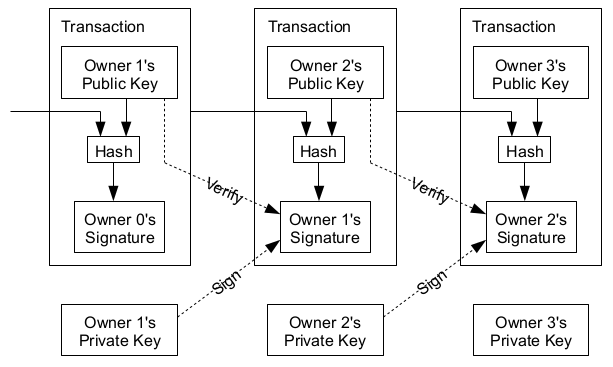
\includegraphics[width=0.7\textwidth]{fig/bitcoin-transfer.png}
    \caption{Transfer from Owner 1 to Owner 2 to Owner 3.
    Image:~\cite{Nakamoto2008bap}.}
  \end{figure}
\end{frame}

%\begin{frame}
%  \begin{figure}
%    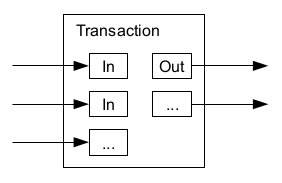
\includegraphics[width=0.4\textwidth]{fig/bitcoin-transaction.png}
%    \caption{A transaction.
%    Image:~\cite{Nakamoto2008bap}.}
%  \end{figure}
%\end{frame}

\subsection{Problems}

\begin{frame}
  \begin{figure}
    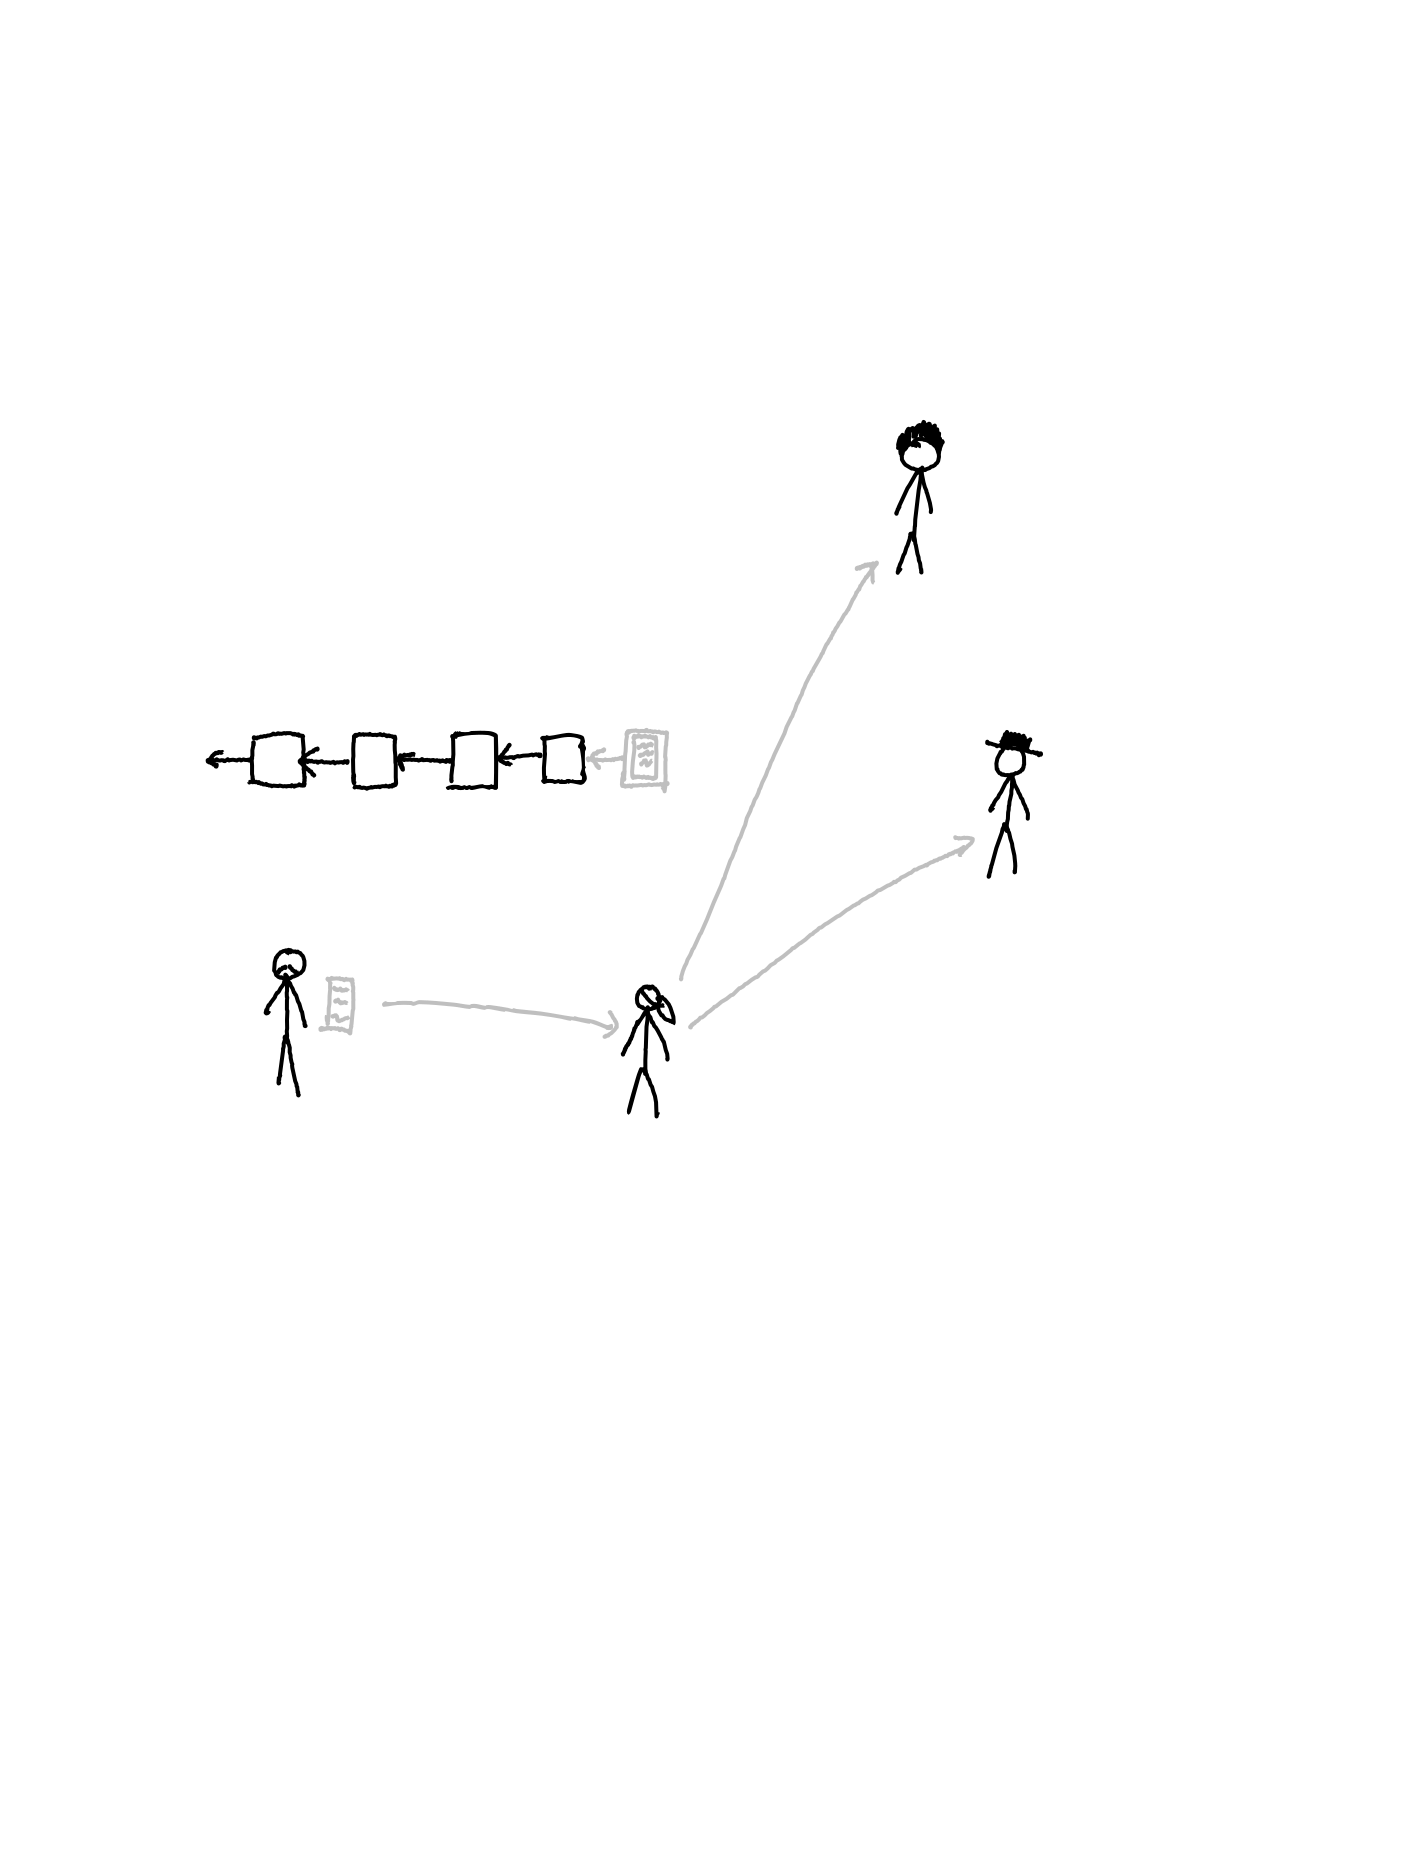
\includegraphics[height=0.8\textheight]{fig/distribute-tx.pdf}
    \caption{Distributing transactions}
  \end{figure}
\end{frame}

\begin{frame}
  \begin{figure}
    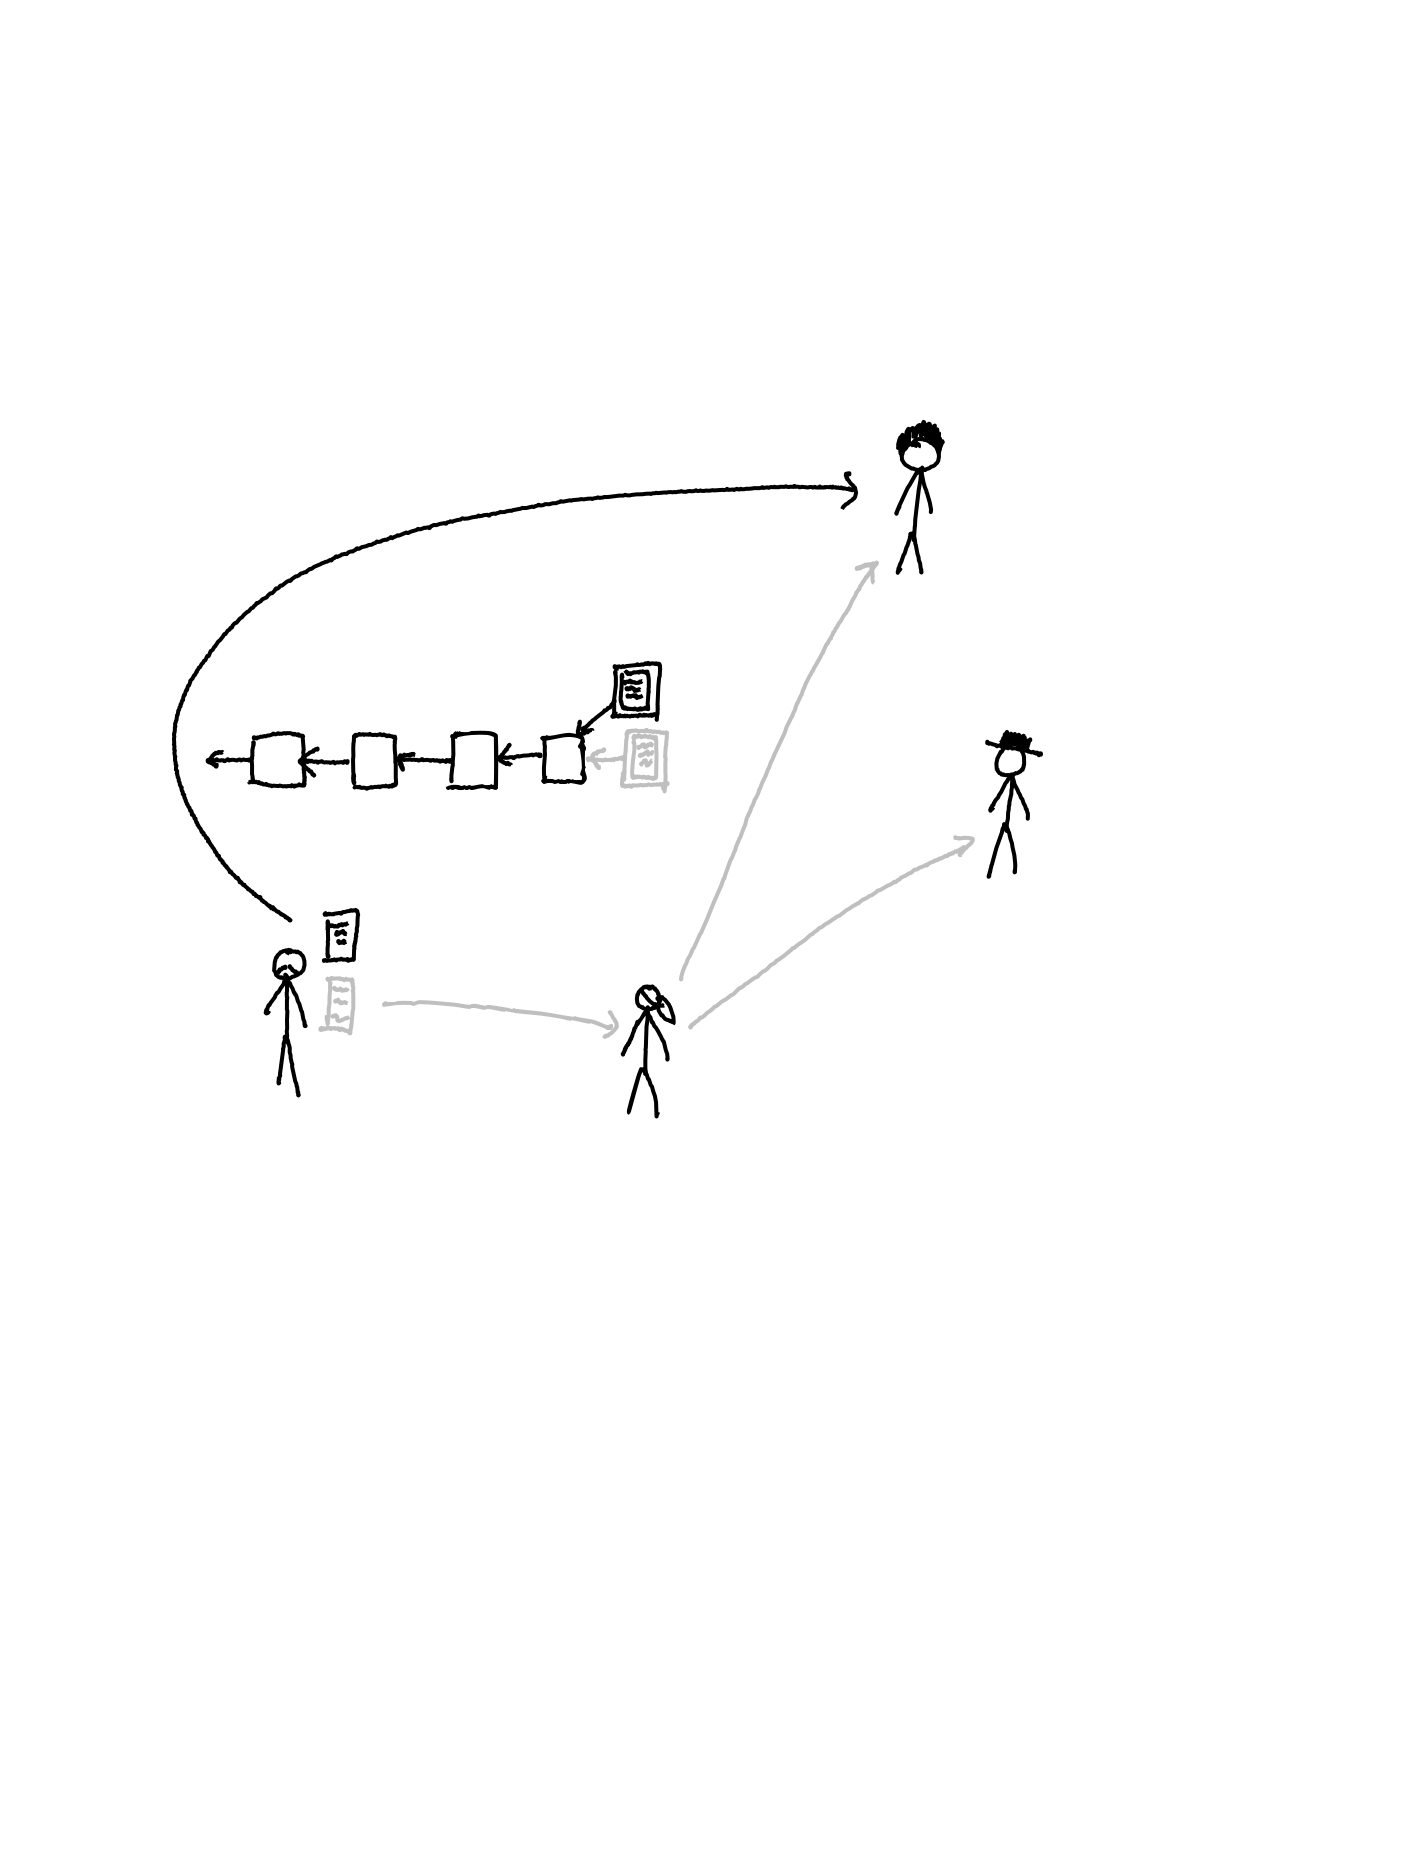
\includegraphics[height=0.8\textheight]{fig/distribute-tx-malicious.pdf}
    \caption{Maliciously distributing transactions}
  \end{figure}
\end{frame}

\begin{frame}
  \begin{figure}
    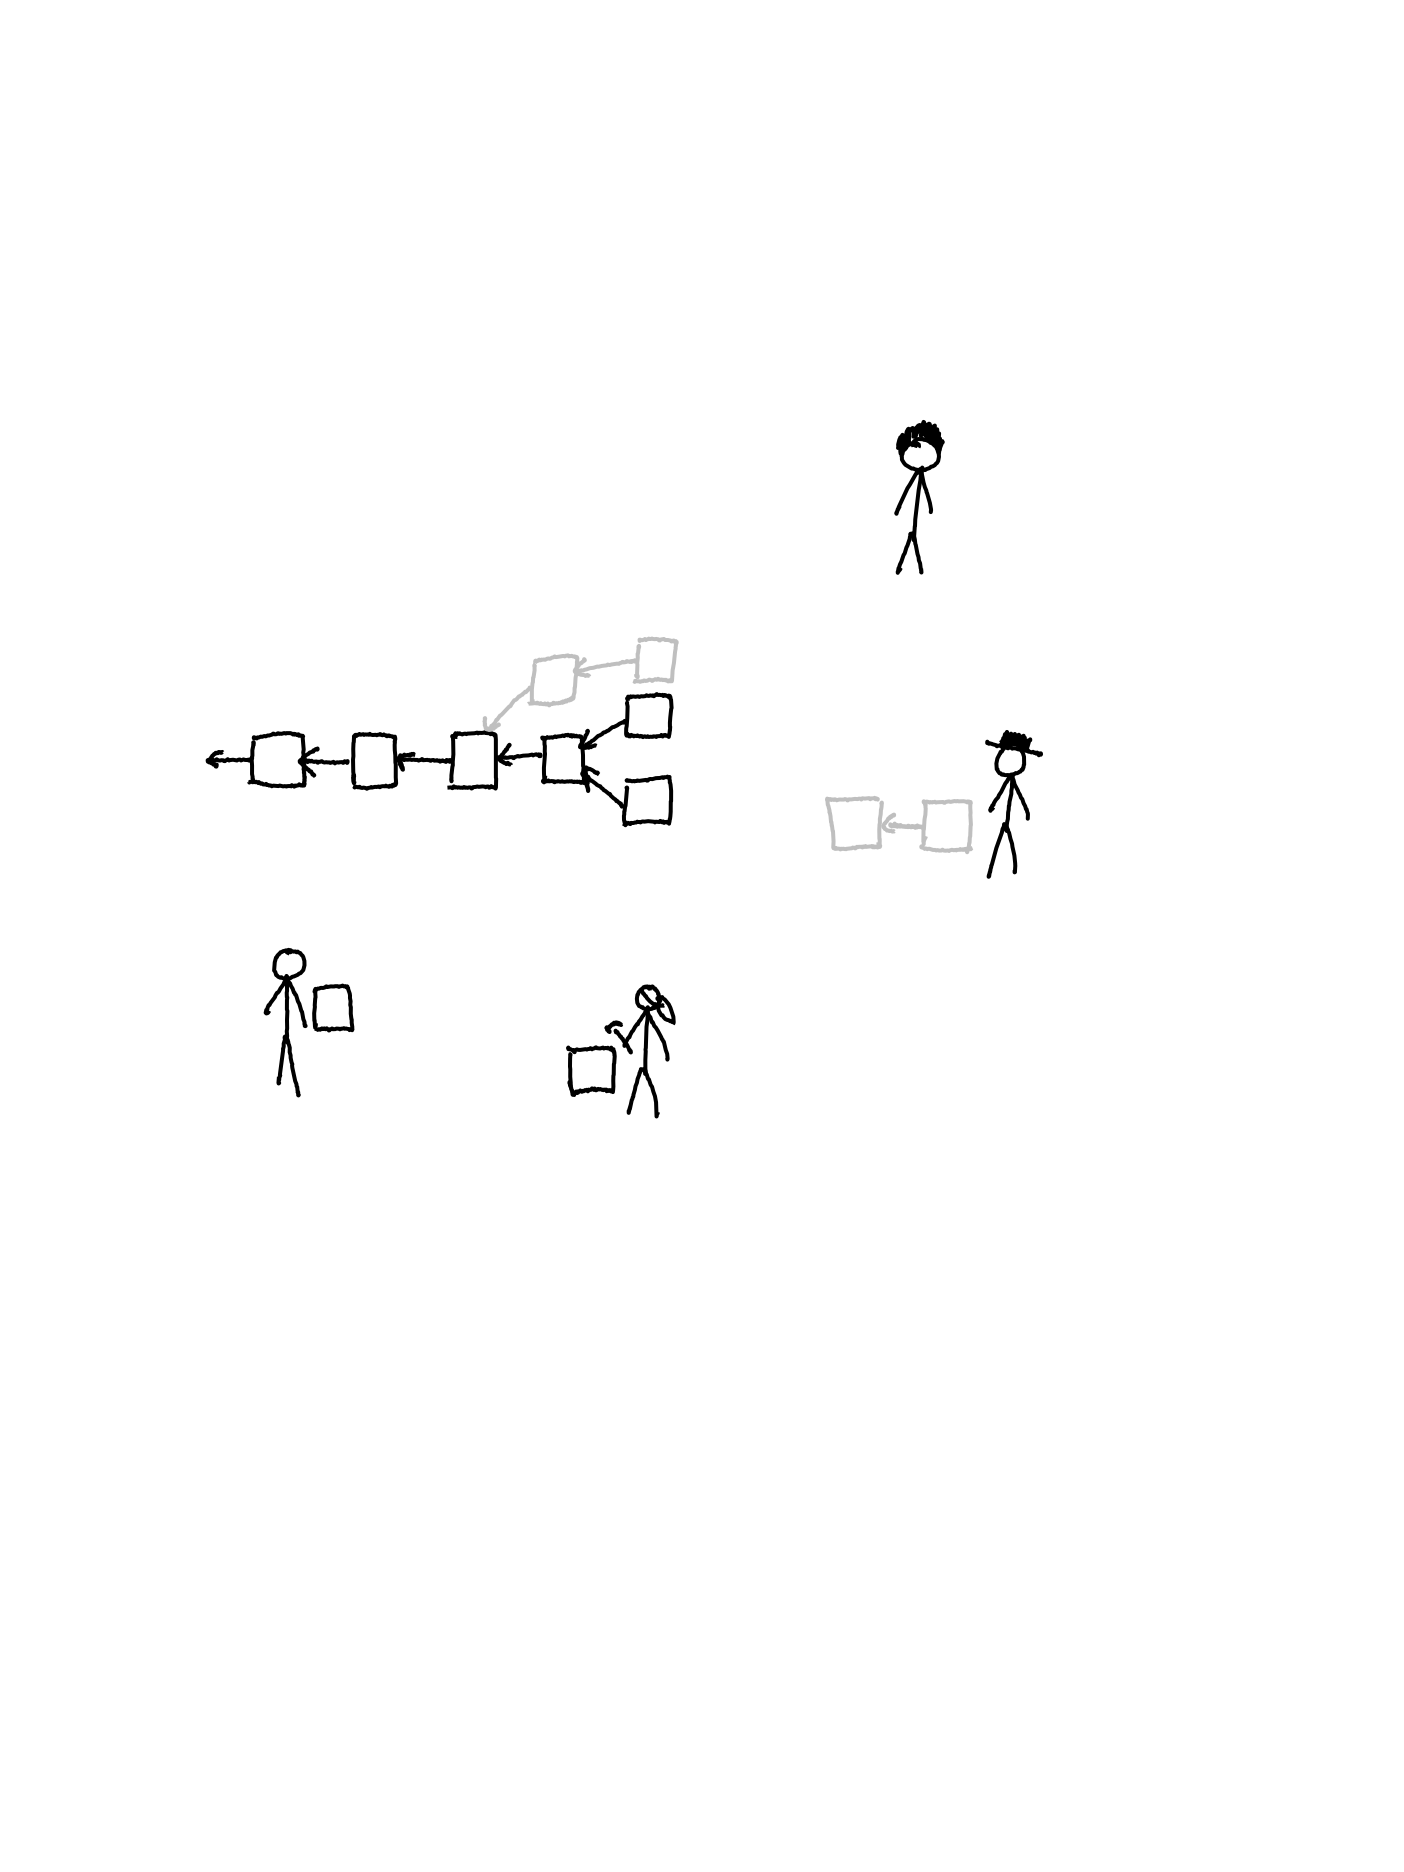
\includegraphics[height=0.8\textheight]{fig/mining.pdf}
    \caption{How a block chain is agreed upon.}
  \end{figure}
\end{frame}

%\begin{frame}
%  \begin{idea}[Piecing together all ideas]
%    \begin{itemize}
%      \item Every transaction is distributed to all participating nodes.
%      \item Each node collects transactions into a block.
%      \item Each node tries to solve the hard problem for the block.
%      \item A block with a solution to the problem is valid.
%      \item Other nodes accept such blocks as the new head of the chain.
%    \end{itemize}
%  \end{idea}
%\end{frame}


\section[Chaining]{Chaining and block chains}

\begin{frame}
  \begin{remark}
    \begin{itemize}
      \item We must order transactions to prevent double spending.
    \end{itemize}
  \end{remark}
\end{frame}

\begin{frame}
  \begin{figure}
    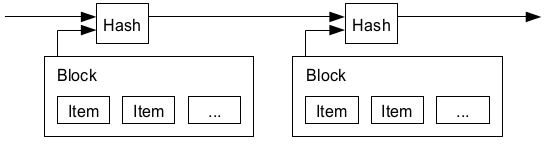
\includegraphics[width=0.7\textwidth]{fig/bitcoin-stamp.png}
    \caption{A simple \enquote{time-stamping} mechanism.
    Image:~\cite{Nakamoto2008bap}.}
  \end{figure}

  \pause

  \begin{remark}
    \begin{itemize}
      \item It's an ordering of the set of transactions.
      \item This is similar to the commit objects in Git.
    \end{itemize}
  \end{remark}
\end{frame}

\begin{frame}
  \begin{figure}
    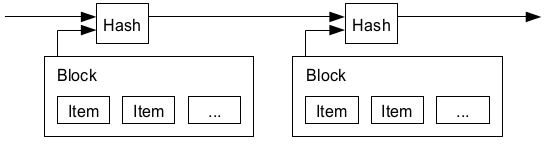
\includegraphics[width=0.7\textwidth]{fig/bitcoin-stamp.png}
    \caption{A simple time-stamping mechanism.
    Image:~\cite{Nakamoto2008bap}.}
  \end{figure}

  \vfill

  \only<1>{%
    \begin{exercise}
      \begin{itemize}
        \item What prevents me from forging a block and claim it was before 
          another block in the time line?
      \end{itemize}
    \end{exercise}
  }
  \only<2>{%
    \begin{solution}
      \begin{itemize}
        \item That block I forge must have the same hash.
        \item I must find a collision.
      \end{itemize}
    \end{solution}
  }
\end{frame}


\section{Proof-of-work}

\begin{frame}
  \begin{question}
    \begin{itemize}
      \item Then why do we need proof-of-work?
    \end{itemize}
  \end{question}

  \begin{remark}
    \begin{itemize}
      \item Because the block chain is not fixed!
    \end{itemize}
  \end{remark}
\end{frame}

%\begin{frame}
%  \begin{question}
%    \begin{itemize}
%      \item How to reach consensus about the chain?
%      \item Why can't one person pretend to be many? (Sybil attack)
%    \end{itemize}
%  \end{question}
%
%  \begin{idea}[Proof-of-work]
%    \begin{itemize}
%      \item We require a difficult problem to be solved.
%      \item We only consider a block if this problem is solved.
%      \item All other details should also check out.
%    \end{itemize}
%  \end{idea}
%\end{frame}

\begin{frame}
  \begin{figure}
    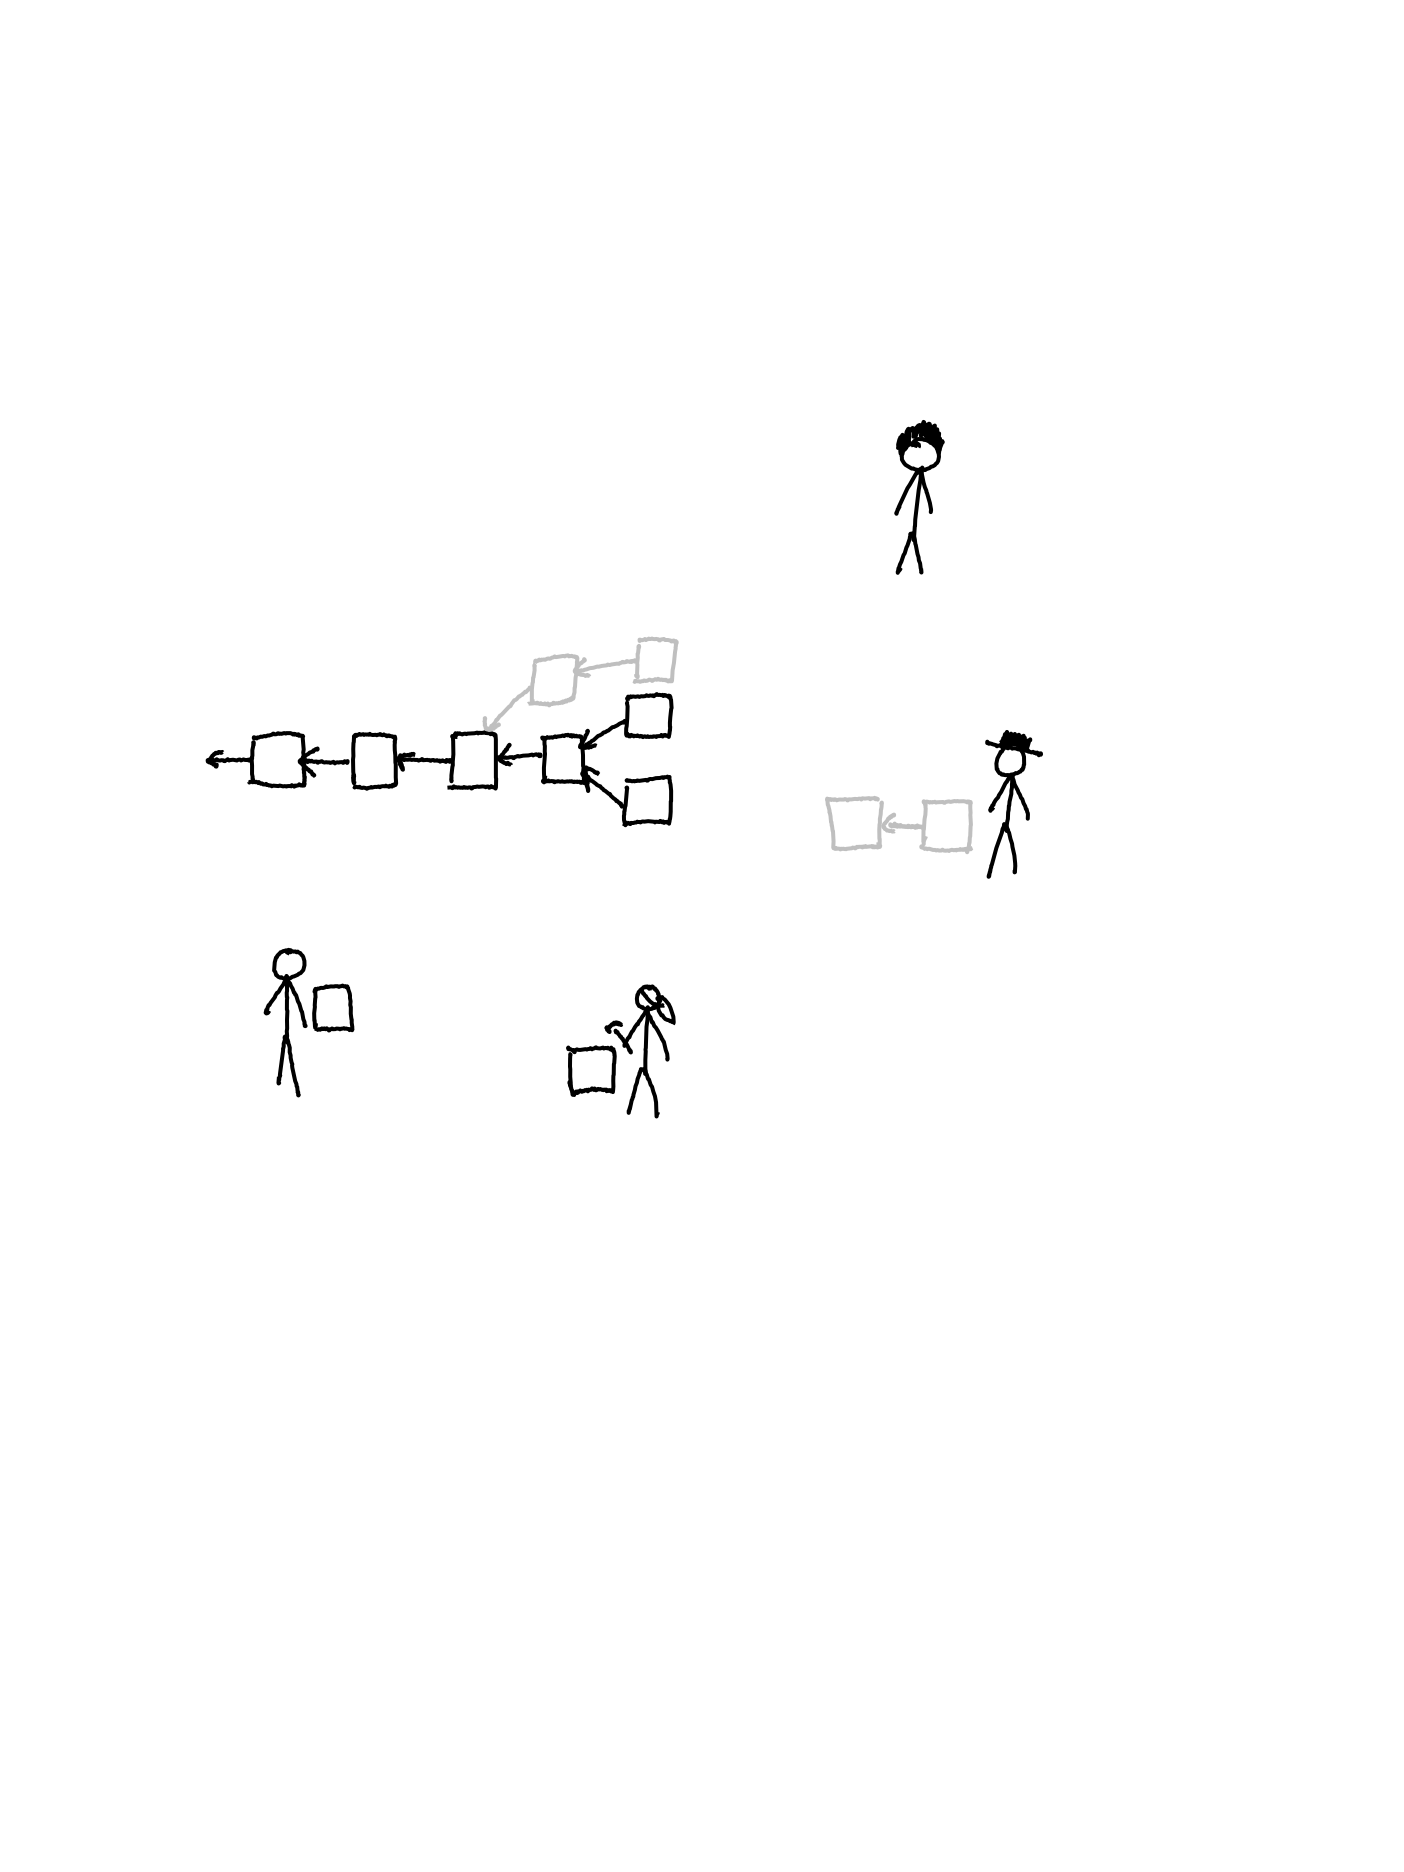
\includegraphics[height=0.8\textheight]{fig/mining.pdf}
    \caption{How a block chain is agreed upon.}
  \end{figure}
\end{frame}

\begin{frame}
  \begin{remark}[Forgery]
    \begin{itemize}
      \item The time stamping above yields \(h_i = h(h_{i-1}\concat b_i)\).
      \item \(h\) is a collision-resistant hash function.
      \item But this can easily be recomputed.
      \item Make the chain the longest and the others accept it as valid.
    \end{itemize}
  \end{remark}

  \begin{question}
    \begin{itemize}
      \item How to fix this problem?
    \end{itemize}
  \end{question}
\end{frame}

\begin{frame}
  \begin{figure}
    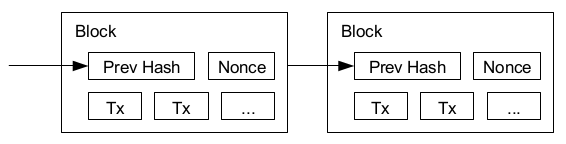
\includegraphics[width=0.7\textwidth]{fig/bitcoin-pow.png}
    \caption{A time-stamping mechanism to prevent forgery.
    Image:~\cite{Nakamoto2008bap}.}
  \end{figure}
  
  \begin{solution}
    \begin{itemize}
      \item \(h_i = h(h_{i-1}\concat b_i\concat n)\),
        where \(n\) is a nonce, \(h_i < k\).
    \end{itemize}
  \end{solution}

  \pause

  \begin{remark}[But this is to solve the preimage problem?!]
    \begin{itemize}
      \item Difficulty~\(k\) is adjusted so that can be solved every 
        10 minutes.
    \end{itemize}
  \end{remark}
\end{frame}

\begin{frame}
  \begin{figure}
    \centering
    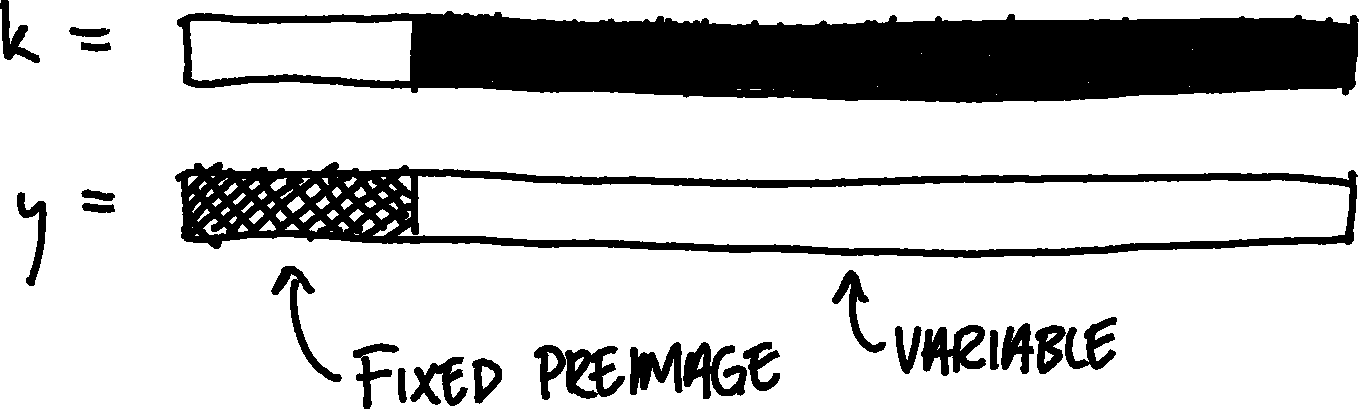
\includegraphics[width=0.8\columnwidth]{fig/pow.pdf}
    \caption{Proof-of-work problem}
  \end{figure}
\end{frame}

\begin{frame}
  \begin{figure}
    \centering
    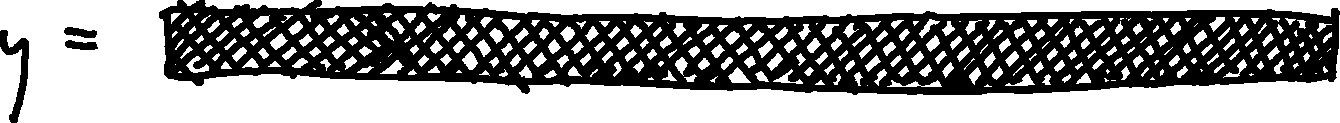
\includegraphics[width=0.8\columnwidth]{fig/preimage.pdf}
    \caption{Preimage problem}
  \end{figure}
\end{frame}

\section{Tree hashing}

\begin{frame}
  \begin{figure}
    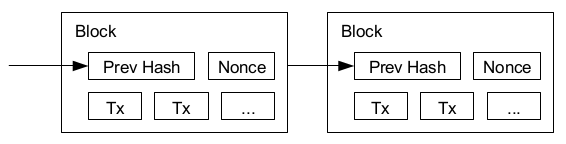
\includegraphics[width=0.7\textwidth]{fig/bitcoin-pow.png}
    \caption{A time-stamping mechanism to prevent forgery.
    Image:~\cite{Nakamoto2008bap}.}
  \end{figure}
\end{frame}

\begin{frame}
  \begin{figure}
    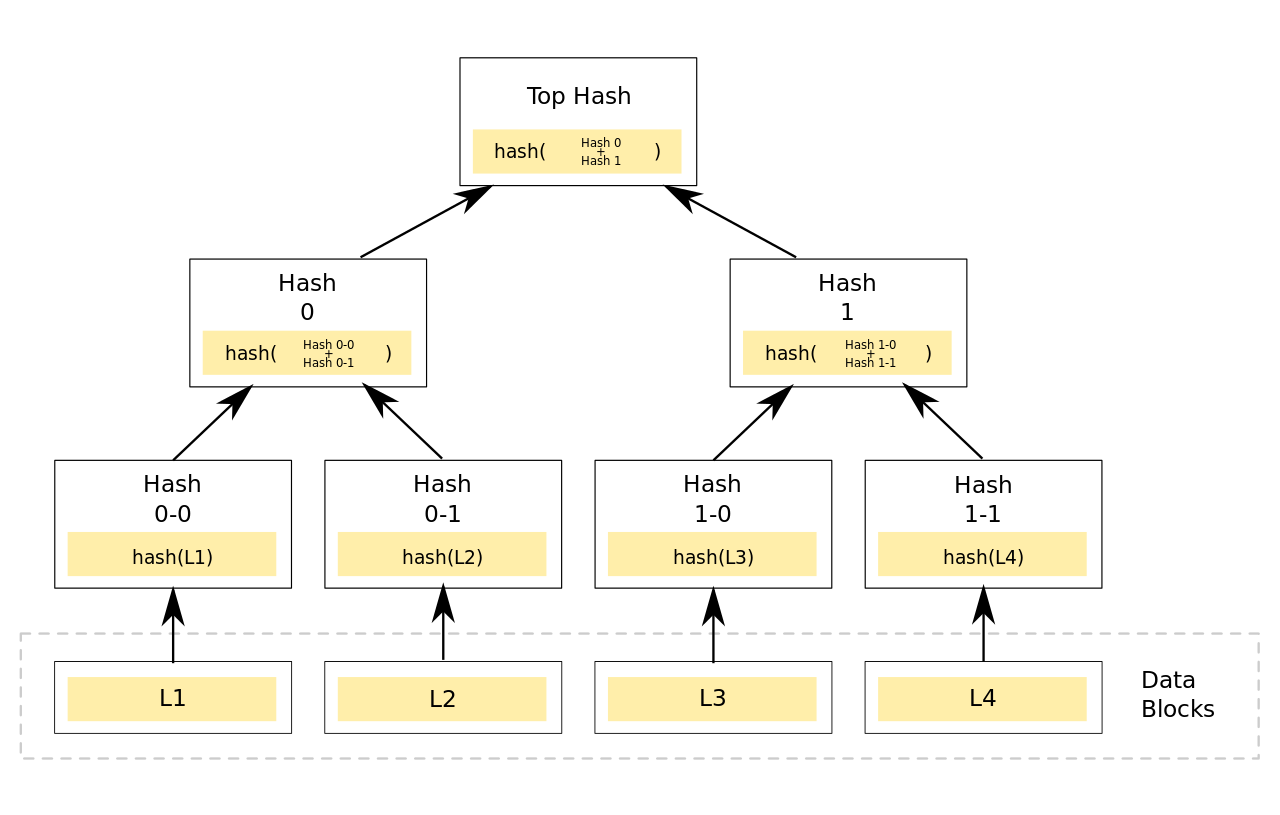
\includegraphics[width=0.9\columnwidth]{fig/merkle-tree.png}
    \caption{Merkle tree}
  \end{figure}
\end{frame}

\begin{frame}
  \begin{figure}
    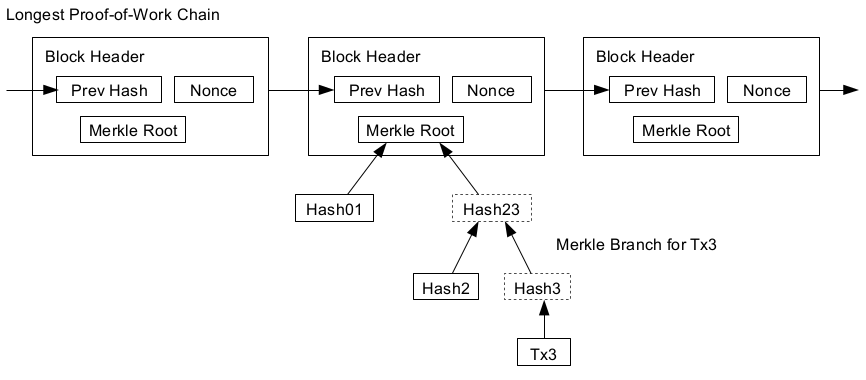
\includegraphics[width=\textwidth]{fig/bitcoin-powchain.png}
    \caption{Merkle trees for transactions.
      Only need Hash01, Hash2 to verify Tx3 is in there.
    Image:~\cite{Nakamoto2008bap}.}
  \end{figure}
\end{frame}

